\documentclass{article}
\usepackage{graphicx} % Required for inserting images
\usepackage{hyperref}
\usepackage{bookmark}
\usepackage[ruled,vlined]{algorithm2e}
\usepackage{listings}
\usepackage{xcolor}
\usepackage{algorithm}
\usepackage{algorithmic}

% Define a nice style for Python code
\lstdefinestyle{pythonstyle}{
    language=Python,
    basicstyle=\ttfamily\small,
    breaklines=true,
    commentstyle=\color{green!60!black},
    keywordstyle=\color{blue},
    stringstyle=\color{red},
    numbers=left,
    numberstyle=\tiny\color{gray},
    backgroundcolor=\color{gray!10},
    frame=single
}

\title{Compte-rendu du projet d'analyse de données: applications au jeu Stardle}
\author{Charles Azais de Vergeron et Octave Feuilland }
\date{Mai 2025}

\begin{document}
\maketitle
\section{Sommaire}
blallalalaal

\newpage
\maketitle
\section{Introduction}
\subsection{Présentation du jeu Stardle}

Le jeu Stardle est un jeu en ligne (\href{https://stardle.net}{stardle.net}) basé sur le jeu Wordle / SUTO. 
Le but est de deviner chaque jour un vaisseau choisi au hasard parmi une liste  d'environ 200 éléments. 

Chaque vaisseau est definit par deux types de caractéristiques: 
\begin{itemize}
    \item Qualitatives
    \begin{itemize}
        \item Fabricant (Manufacturer)
        \item Type
        \item Role 
        \item Année d'apparition (Relese Date)
        \item En Jeu ou Non (Status)
    \end{itemize}
    \item Quantitatives
    \begin{itemize}
        \item Nombre de personnes dans l'équipage (Crew)
        \item Valeur en \$ (Price)
        \item Valeurs en monnaie du jeu (Price In game)
        \item Capacité en tant que cargo (Cargo Capacity)
        \item Vitesse de croisière (SCM) et maximale (Max)
        \item Longeur (Length), Largeur (Beam) et Hauteur (Height)
    \end{itemize}
\end{itemize}

Voici un exemple de partie du jeu :
\\
\begin{figure}[ht]
    \centering
    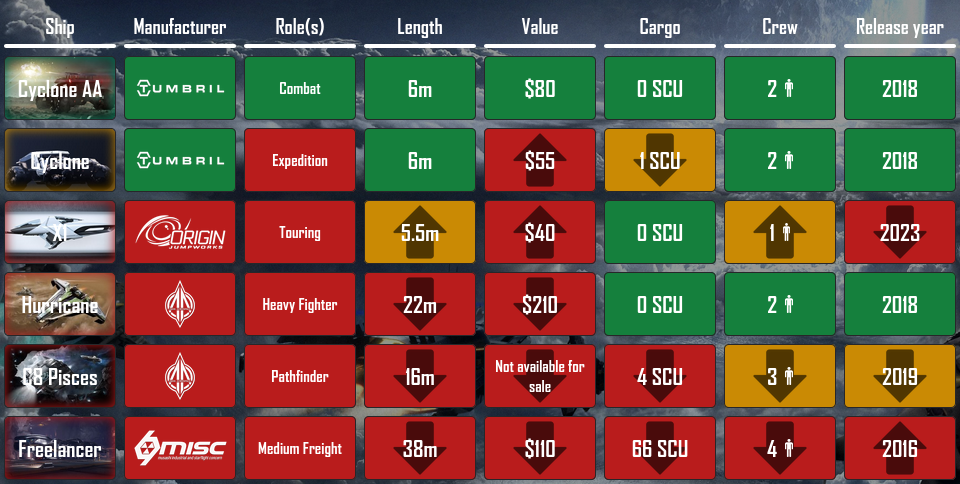
\includegraphics[width=0.8\textwidth]{stardle.png}
    \caption{Exemple d'une partie du jeu Stardle}
    \label{fig:stardle_example}
\end{figure}

Nous avons 3 possibilités de résultats: Vrai, Faux ou Proche (uniquement pour les caractéristiques quantitatives). \\ 

\subsection{Objectif du projet}

L'objectif de ce projet est d'analyser les données du jeu Stardle afin de créer un algorithme capable de trouver  un vaisseau pris au hasard dans la base de données en un minimum de tentatives et de déterminer une combinaison d'essais de vaisseaux qui permet de minimiser le nombre de tentatives.
\\
Nous avons donc récupéré les données, recréé le jeu puis essayé de trouver un 
algorithme optimal pour déterminer le vaisseau le plus efficacement possible. 

\maketitle
\section{Récupération des données}

La récupération des données est faite via le script Python \verb|CreateShipDatabase.py|.
Ce script utilise l'API officielle de \href{https://starcitizen.tools/}{Star Citizen Wiki}  pour récupérer les informations sur les vaisseaux.

\subsection{Structure du script}
Le script de collecte de données se décompose en plusieurs étapes principales :
\begin{enumerate}   
    \item \textbf{Collecte des données} \\
        Nous utilisation l'API \verb|https://api.star-citizen.wiki/| pour obtenir la liste complète des 
        vaisseaux.
        Pour chaque vaisseau, le script récupère les données via l'API et 
        extrait toutes les caractéristiques -- dans la configuration "All" -- 
        et uniquement celles du jeu Stardle -- dans la configuration  "Stardle" -- cf le code de \verb|CreateShipDatabase.py| \newline
        Dans la suite du rapport, "Stardle" désigne la configuration du jeu et "All" la configuration complète.
    \item \textbf{Stockage des données}
    
    \begin{itemize}
        \item Création de deux fichiers JSON :
        \begin{itemize}
            \item \verb|shipList.json| : liste des vaisseaux et leurs liens
            \item \verb|shipDB_All.json| : base de données complète des vaisseaux
            \item \verb|shipDB_Stardle.json| : base de données avec les catégories du jeu Stardle 
        \end{itemize}
    \end{itemize}
\end{enumerate}

\section{Nettoyage et préparation des données}

Pour ajouter de la complexité, nous avons mélangés les deux base de données.
Stardle est la base du projet. Nous avons extrait de "All" les valeurs de scm,max, length, beam. Nous avons aussi 
rajouté une colonne "price in game" qui correspond à la valeur du vaisseau dans le jeu (via le site 
\href{https://www.erkul.games/live/calculator}{Erkul.com})
\newline
Pour la gestion des valeurs manquantes, nous avons étudié les dépendances entre les colonnes.
Nous avons remarqué que certaines colonnes étaient très corrélées entre elles. Par exemple, le prix \$ (sans valeurs manquantes) 
et celle du prix en jeu (avec beaucoup des valeurs manquantes). Nous avons tenté de remplr les valeurs manquantes
en utilisant une regression lineaire et une regression quadratique mais ce ne fut pas concluant. 
Nous avons donc appliqué l'algorithme suivant: \\

\begin{algorithm}[H]
    \SetAlgoLined
    \KwData{CSV avec valeurs manquantes aux colonnes status,type,manufacturer}
    \KwResult{Colonne sans valeurs manquantes}
    groupby by status,type,manufacturer\;
    \For{vaisseaux in names}{
        \eIf{mean(groupby by status,type,manufacturer) $\neq$ Nan \textbf{and} price\_in\_game == 0}{
            price\_in\_game[vaisseaux] = mean(groupby by status,type,manufacturer)\;
        }{
            price\_in\_game[vaisseaux] = mean\;
        }
    }
\end{algorithm}
\newline
\section{Algorithme de jeu}

Dans un premier temps, nous avons pensé à une dichotomie en utilisant le script du jeu pour un utilisateur.
Cependant, la théorie des graphes s'appliquaient assez bien à notre problème.  
Nous avons crée un graphe dont les vaisseaux sont les noeuds et la distance entre eux : \\
Si la marque ou le nombre d'équipage ou le type ou le role ou la date de sortie ou le statut sont differents,
la distance augmente de 1 (choix arbitraire). Puis nous prennons la racine carrée. C'est donc comparable à une distance euclidienne binaire: cf \verb|detailed_paths_history.csv| pour avoir toutes les distances.\\
Cela nous donne le graphe suivant pour les types des vaisseaux :

\ref{fig:graph}
\begin{figure}[h]
    \centering
    \includegraphics[width=0.9\textwidth]{graphe_type.png}
    \caption{Exemple d'une partie du jeu Stardle}
    \label{fig:graph}
\end{figure}
\\
Nous considerons l'équipage et l'année de sortie comme des données qualitatives car elles sont discrètes et non 
continues comme peuvent l'être la masse ou le prix par exemple. 

\subsection{Algorithme Stardle Auto}

L'algorithme \texttt{stardle\_auto()} est une version automatisée du jeu Stardle qui utilise une approche basée sur les distances entre vaisseaux pour optimiser la recherche. Voici son fonctionnement :

\begin{algorithm}[H]
\SetAlgoLined
\KwData{Base de données des vaisseaux, Matrice des distances pré-calculées}
\KwResult{Nombre de tentatives et liste des vaisseaux essayés}

verifier\_ship retourne les informations comparatives entre deux vaisseaux. 
\newline
get\_ship\_distance retourne la distance entre deux vaisseaux depuis la matrices des distances.
\newline
ship\_secret $\leftarrow$ Choisir un vaisseau aléatoire dans la base\_de\_données 
\newline
tentatives\_max $\leftarrow$ 6 
\newline
visited\_ships $\leftarrow$ liste vide
\newline
current\_ship $\leftarrow$ Choisir un vaisseau aléatoire initial

\For{essais de 1 à tentatives\_max}{
    Ajouter current\_ship à visited\_ships\; \\
    resultat $\leftarrow$ verifier\_ship(ship\_secret, current\_ship)\;\\
    \eIf{resultat == "Bravo"}{
        \Return{(attempt, visited\_ships)}\;
    }{
        closest\_ships $\leftarrow$ [ ]\;\newline
        \For{ship dans base\_de\_données}{
            \If{ship $\notin$ visited\_ships}{
                distance $\leftarrow$ get\_ship\_distance(ship, ship\_secret)\;\\
                \If{distance $\neq$ None}{
                    Ajouter (ship, distance) à closest\_ships\;
                }
            }
        }
        \eIf{closest\_ships non vide}{
            Trier closest\_ships par distance croissante\;
            current\_ship $\leftarrow$ closest\_ships[0]\;
        }{
            current\_ship $\leftarrow$ Choisir aléatoirement parmi les vaisseaux non visités\;
        }
    }
}
\Return{(tentatives\_max + 1, visited\_ships)}\;
\end{algorithm}
\\

\section{Conclusion}

Nous avons consruit un dataset pour jouer au jeu Stardle et créer un alghorithme joueur. Nous voulions détérminer un choix optimal de vaisseau de départ. Cependant, l'alghorithme détérmine le bon vaisseaux en deux essais. De plus, dans certains cas de vaisseaux proches trop égaux dans leur données, l'alghorithme ne les trouve pas (5 cas sur 5000 tentatives ). 
\end{document}